\chapter{Implementação e resultados}
\label{cap:implementacaoresultados}

Neste capítulo será detalhado a implementação, com a configuração do \ac{OS}, do ambiente virtualizado e das ferramentas que irão compôr o
\textit{cluster} de alta disponibilidade. Posteriormente, serão efetuados testes e medições de resultados.

Nas próximas seções será demonstrado a configuração das ferramentas do ambiente de alta disponibilidade, do ambiente de virtualização e 
também do sistema operacional.

Descrever o que nao deu certo no projeto com o ganeti??

\section{Topologia}

A estrutura física adotada está representada na Figura \ref{fig:projeto_fisico}.
Pode-se observar os dois servidores ligados a um \textit{switch} através de dois cabos UTP cada servidor para redundância do cabeamento.
Esta será a estrutura necessária para implementar o \textit{cluster} de alta disponibilidade.

\begin{figure}[h!]
 \centering
 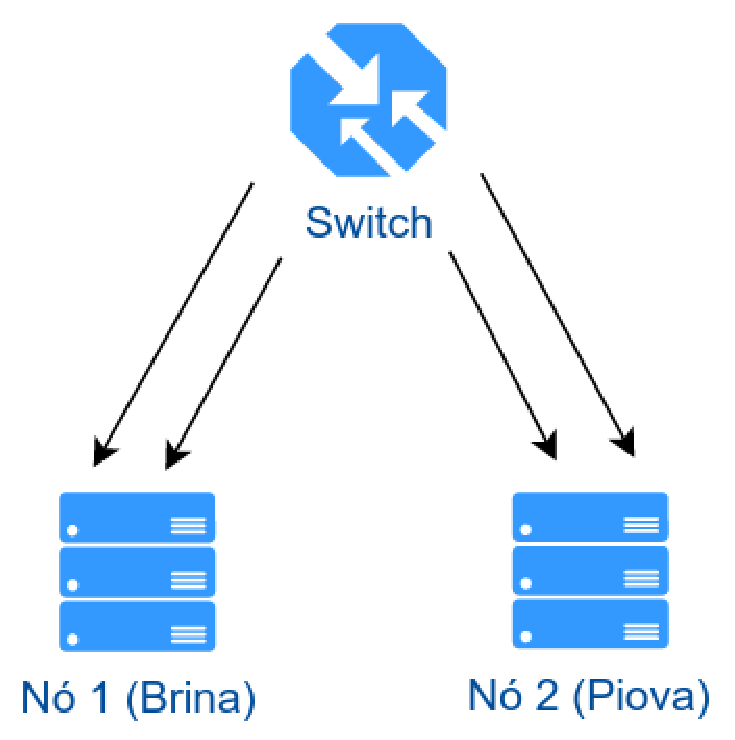
\includegraphics[width=180px]{img/projeto_fisico.eps}
 \caption{Estrutura física.}
 \label{fig:projeto_fisico}
\end{figure}

Na Figura \ref{fig:servidores_brina_piova} tem-se a imagem dos servidores, o primeiro no topo da imagem, \textit{Brina} 
(\textit{Dell PowerEdge 2950}), e o servidor mais abaixo, \textit{Piova} (\textit{Dell PowerEdge R410}).

\begin{figure}[h!]
 \centering
 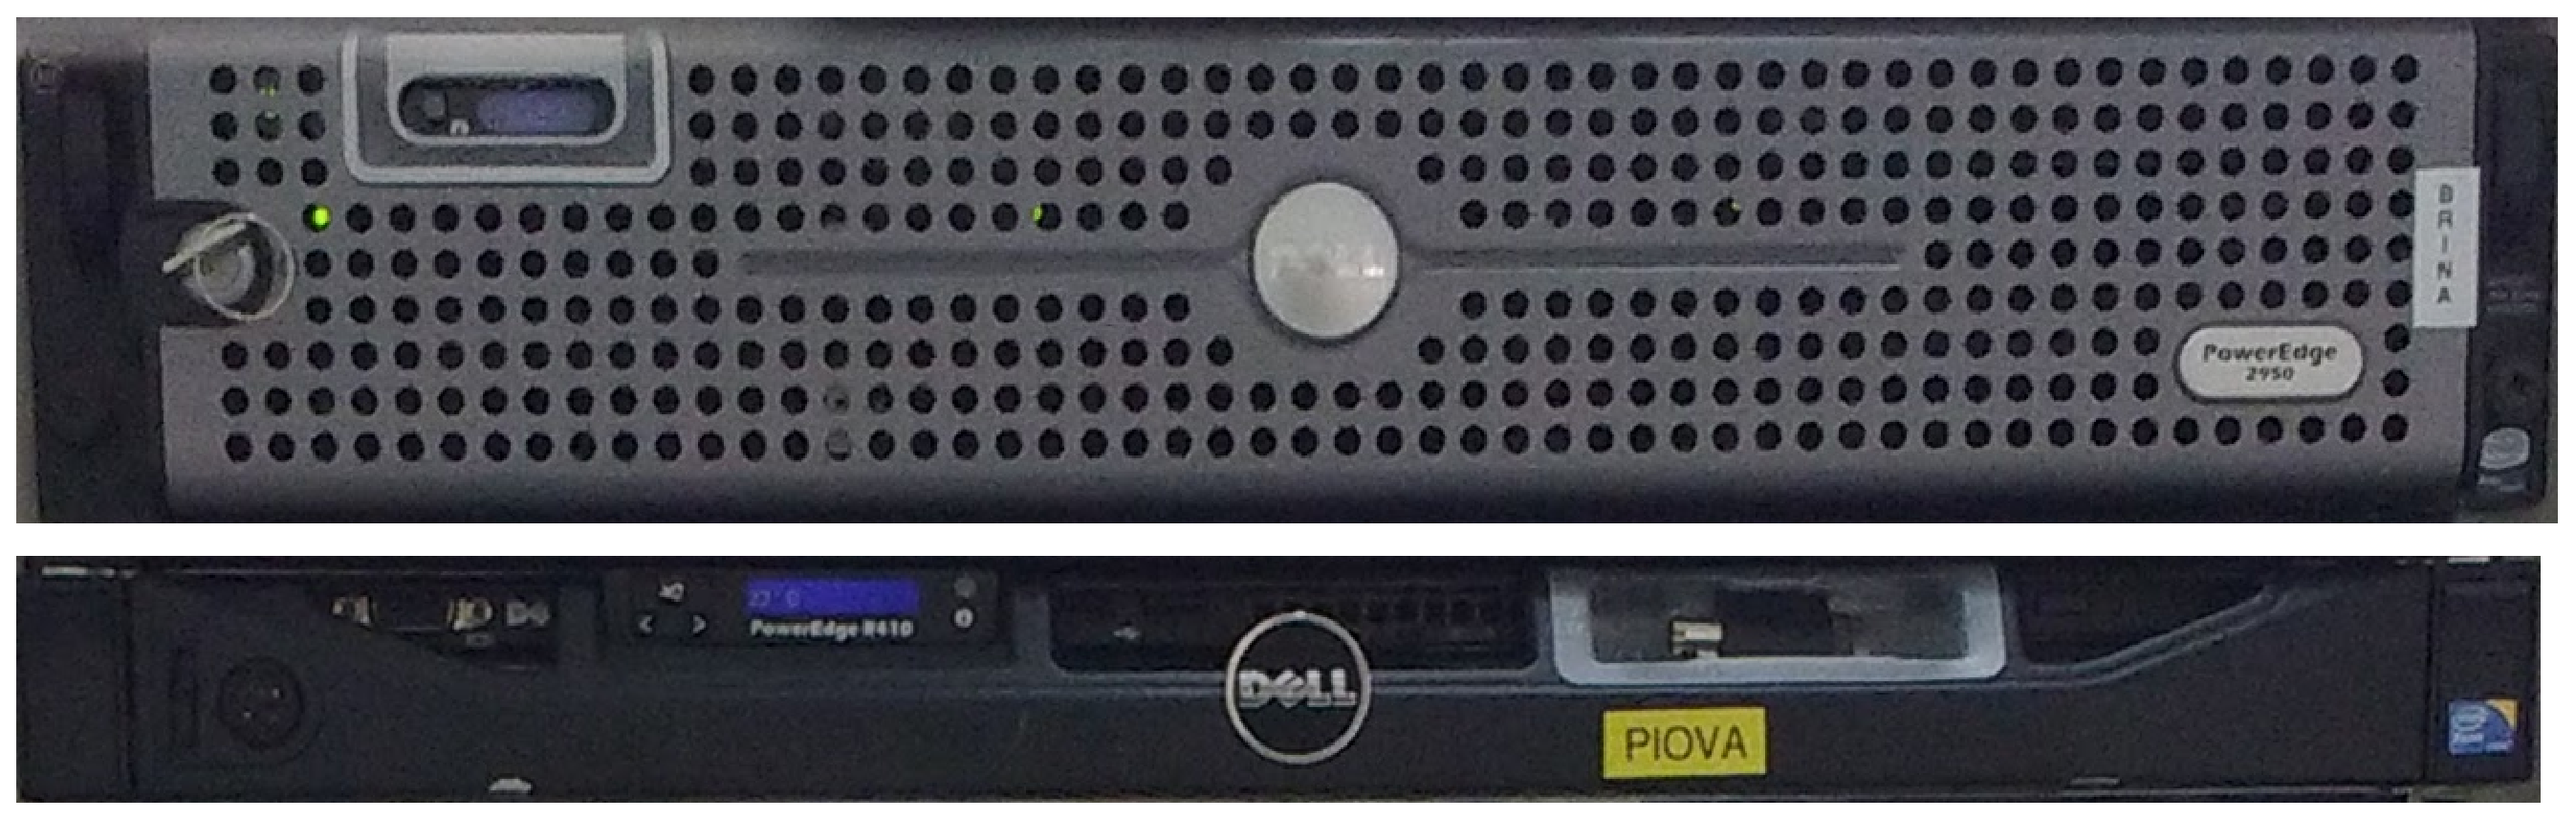
\includegraphics[width=300px]{img/servidores_brina_piova.eps}
 \caption{Servidores.}
 \label{fig:servidores_brina_piova}
\end{figure}

Pode ser observado na Figura \ref{fig:projeto_estrutura} a estrutura que representa a configuração dos \textit{softwares}. Nesta tem-se o 
\textit{software} de gerenciamento do cluster, que fará o monitoramento, iniciará e parará os recursos dos nós, o \textit{software} de replicação 
de dados, o sistema de arquivos, as máquinas virtuais e os serviços localizados nestas máquinas.

\begin{figure}[h!]
 \centering
 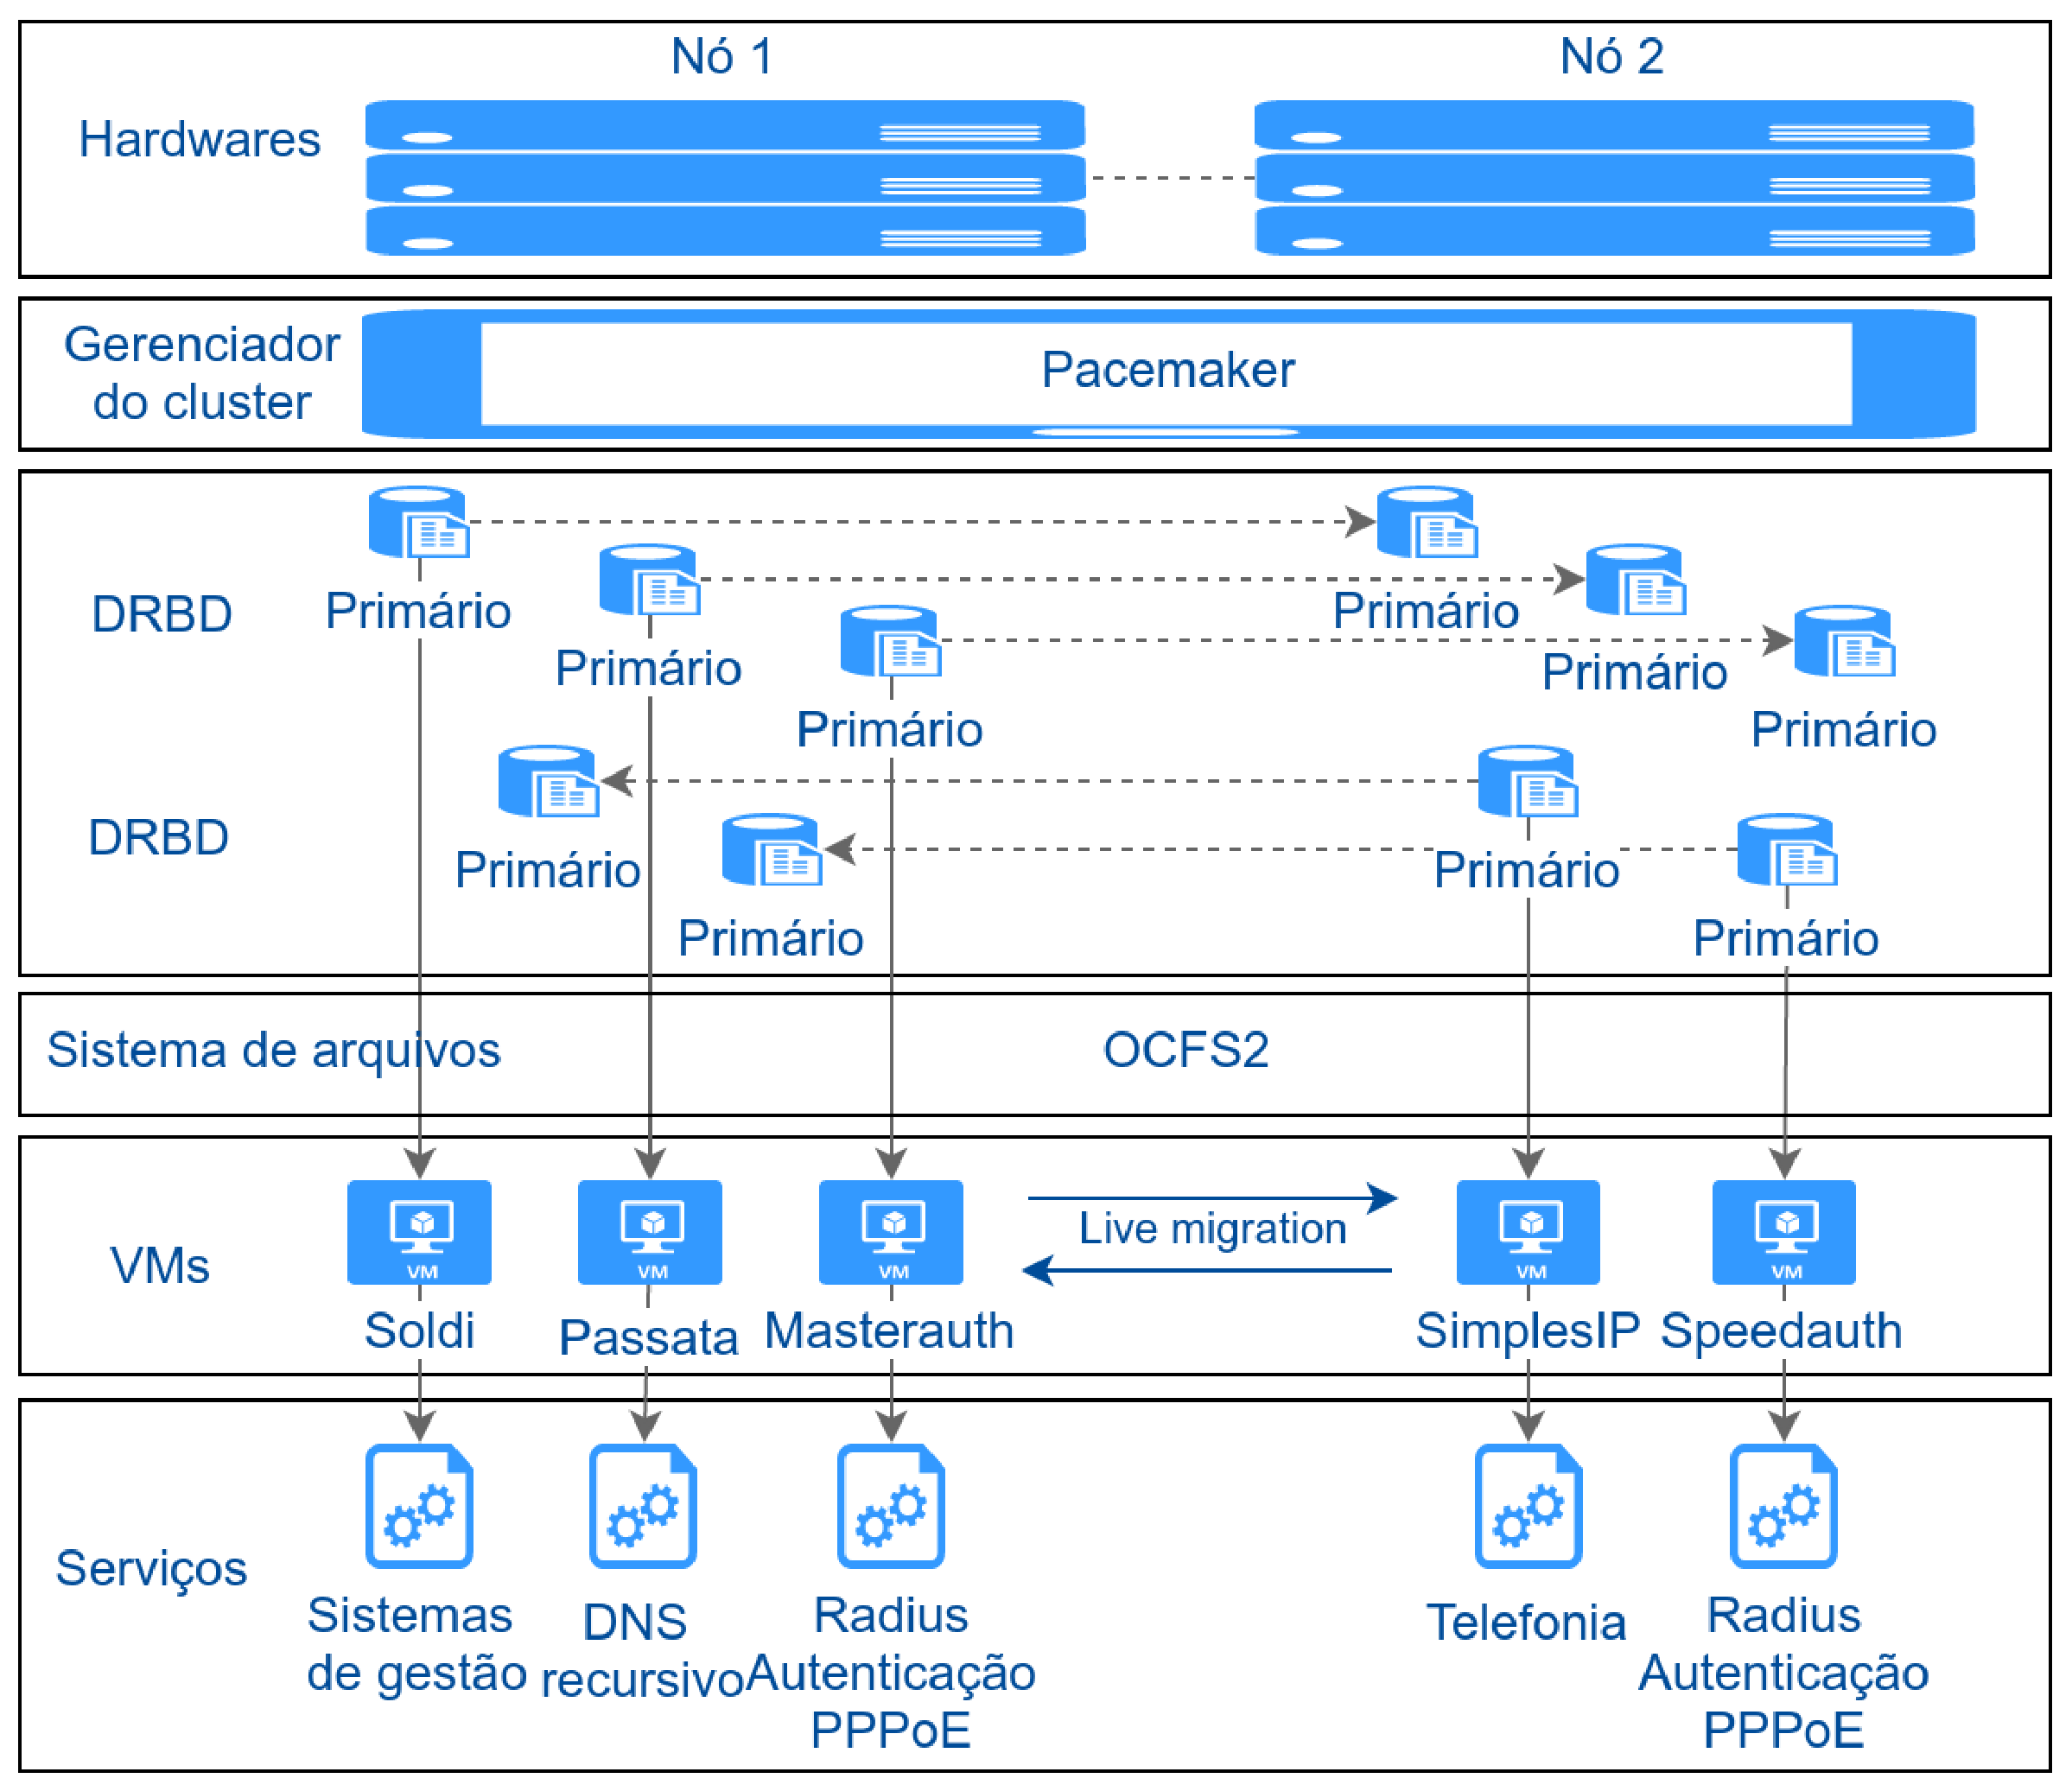
\includegraphics[width=350px]{img/projeto_estrutura.eps}
 \caption{Estrutura do \textit{cluster}.}
 \label{fig:projeto_estrutura}
\end{figure}

tabela com ips??
node 1 brina 192.168.3.1
node 2 piova 192.168.3.2

\section{Configuração do \ac{OS}}

Foi feita a instalação do sistema operacional \textit{Ubuntu 14.04 \ac{LTS}} nos dois servidores. A configuração feita foi a básica do sistema,
com nome do servidor, configuração de rede, localização e instalação do servidor \ac{SSH}.
Além disso, é feito as configurações padrões adotadas pela empresa, como por exemplo, ferramentas de monitoramento, atualização automática
e \textit{firewall}.

\section{Configuração de rede}

Uma forma de incluir as máquinas virtuais a uma rede é através da criação de uma \textit{bridge}. A instalação é feita através do comando:
\begin{lstlisting}[language=bash]
  $ apt-get install bridge-utils
\end{lstlisting}

Além disso, é necessário instalar e configurar o \textit{link aggregation}, o \textit{Ubuntu} usa o padrão \textit{IEEE 802.3ad}. A configuração 
é feita no servidor e no \textit{switch}. Abaixo tem-se os comandos para instalação do \textit{link aggregation}, o primeiro comando faz a 
instalação e o segundo comando carrega o modulo \textit{bonding} no \textit{kernel}:
\begin{lstlisting}[language=bash]
 $ apt-get install ifenslave-2.6
 $ sh -c 'grep -q bonding /etc/modules || echo bonding >> /etc/modules'
\end{lstlisting}

Para a configuração do \textit{link aggregation} deve-se criar uma interface \textit{bond} e nela inclui-se as duas interfaces físicas.
Abaixo tem-se a configuração de rede, que inclui o \textit{link aggregation} e a \textit{bridge}, esta configuração deve ser colocada no 
arquivo \textit{/etc/network/interfaces}:
\begin{lstlisting}
auto eth0
iface eth0 inet manual
bond-master bond0

auto eth1
iface eth1 inet manual
bond-master bond0

auto bond0
iface bond0 inet manual
       bond-mode 4
       bond-slaves eth0 eth1
       bond-lacp-rate 1
       bond-miimon 100
       bond-xmit_hash_policy layer3+4

auto br0
iface br0 inet static
       address x.x.x.x
       netmask 255.255.255.0
       network x.x.x.0
       broadcast x.x.x.255
       gateway x.x.x.x
       dns-nameservers 8.8.8.8 8.8.4.4
       
       bridge_ports bond0
       bridge_stp off
       bridge_maxwait 0
\end{lstlisting}

Também será necessário configurar algumas \textit{vlans} para algumas máquinas virtuais. Os comandos a seguir farão a instalação e carregarão
o modulo do \textit{kernel} necessário para gerenciar \textit{vlans}:
\begin{lstlisting}[language=bash]
 $ apt-get install vlan
 $ sudo  sh -c 'grep -q 8021q /etc/modules || echo 8021q >> /etc/modules'
 $ sudo modprobe 8021q
\end{lstlisting}

\section{Configuração de disco}

Os discos que serão replicados podem ser utilizados diretamente no \ac{DRBD} (por exemplo \textit{/dev/sda2}) ou configurados com \ac{LVM}. Adotou-se
a configuração utilizando \ac{LVM} pois torna-se mais fácil a manipulação dos discos. O comando abaixo faz a criação de um volume lógico chamado 
\textit{lvdrbd} com tamanho de 500 GB, este volume pertence ao grupo de volumes \textit{vg0}.
\begin{lstlisting}[language=bash]
 $ lvcreate -n lvdrbd vg0 -L 500G
\end{lstlisting}

\subsection{DRBD}

Para a instalação do \textit{software} de replicação de dados é necessário instalar os dois pacotes, que estão listados abaixo:
\begin{lstlisting}[language=bash]
 $ apt-get install drbd8-utils drbdlinks
\end{lstlisting}

É necessário alterar a configuração global do \ac{DRBD} que está localizada em \textit{/etc/drbd.d/global\_common.conf}:
\begin{lstlisting}
global {
        usage-count yes;
        minor-count 16;
}
\end{lstlisting}

Posteriormente, deve-se criar um recurso que definirá os dispositivos de disco, os endereços \ac{IP} e portas dos servidores.
Deve-se criar o arquivo \textit{/etc/drbd.d/vms.res}, o qual armazenará essa configuração:
\begin{lstlisting}
 resource vms {
    meta-disk internal;
    device /dev/drbd0;
    protocol C;
    disk {
        fencing resource-only;
        resync-rate 50M;
    }
    handlers {
        fence-peer "/usr/lib/drbd/crm-fence-peer.sh";
        after-resync-target "/usr/lib/drbd/crm-unfence-peer.sh";
    }
    net {
        allow-two-primaries;
    }
    startup {
        become-primary-on both;
    }
    on brina {
        address x.x.x.x:7791;
        disk /dev/vg0/lvdrbd;
    }
    on piova {
        address x.x.x.x:7791;
        disk /dev/vg0/lvdrbd;
    }
}
\end{lstlisting}
Explicar os opcoes??

Para o funcionamento correto dessa ferramenta, o nome dos servidores (localizado em \textit{/etc/hostname}) deve ser exatamente igual a opção
\textit{on} da configuração do recurso.

Após ter sido feita a configuração do \ac{DRBD}, deve-se reiniciar o serviço para aplicá-la:
\begin{lstlisting}[language=bash]
 $ service drbd restart 
\end{lstlisting}

Deve-se inicializar os discos do \ac{DRBD}, primeiro comando, e subi-lo para conectar ao outro nó, segundo comando. Após isso deve-se eleger
os nós como primário e sincronizar os seus dados, terceiro comando:
\begin{lstlisting}[language=bash]
 $ drbdadm create-md vms
 $ drbdadm up vms
 $ drbdadm -- --overwrite-data-of-peer primary vms
\end{lstlisting}

E por fim pode-se verificar o estado dos recursos do \ac{DRBD} através do comando:
\begin{lstlisting}[language=bash]
 $ service drbd status
\end{lstlisting}

\subsection{OCFS2}

O \ac{OCFS2} é um sistema de arquivos para \textit{cluster}, ele faz o gerencimento de \textit{locks} que é necessário para o funcionamento 
do \textit{Pacemaker}. Para sua instalação é necessário um pacote que está sendo instaldo abaixo:
\begin{lstlisting}[language=bash]
 $ apt-get install ocfs2-tools
\end{lstlisting}

É preciso fazer duas configurações, a primeira para criar o \textit{cluster}, localizada no arquivo \textit{/etc/ocfs2/cluster.conf}:
\begin{lstlisting}
node:
        ip_port = 7777
        ip_address = x.x.x.x
        number = 0
        name = brina
        cluster = clusterocfs
node:
        ip_port = 7777
        ip_address = x.x.x.x
        number = 1
        name = piova
        cluster = clusterocfs
cluster:
        node_count = 2
        name = clusterocfs
\end{lstlisting}

A segunda configuração é feita no arquivo \textit{/etc/default/o2cb}, ela faz o carregamento do \textit{driver} no \textit{boot} e a definição 
do nome do cluster para inicialização:
\begin{lstlisting}
O2CB_ENABLED=true
O2CB_BOOTCLUSTER=clusterocfs
\end{lstlisting}

Para aplicar as configurações deve-se reiniciar o serviço:
\begin{lstlisting}[language=bash]
 $ service ocfs2 restart
\end{lstlisting}

E por fim, deve-se construir o sistema de arquivos no dispositivo criado pelo \ac{DRBD}, através do comando:
\begin{lstlisting}[language=bash]
 $ mkfs.ocfs2 /dev/drbd/by-res/vms
\end{lstlisting}

%bug ocfs2
Na versão 1.6.4 do pacote \textit{ocfs2-tools} no \textit{Ubuntu 14.04} há um \textit{bug}\footnote{Detalhes do \textit{bug}: 
https://bugs.launchpad.net/ubuntu/+source/ocfs2-tools/+bug/1412438} que impede o \textit{Pacemaker} de montar o sistema de arquivo \ac{OCFS2}. 
Para corrigi-lo deve aplicar o \textit{patch} abaixo no arquivo \textit{/usr/lib/ocf/resource.d/heartbeat/Filesystem}:
\begin{lstlisting}
--- Filesystem 2013-12-16 07:41:25.000000000 +0000
+++ Filesystem.new 2015-01-19 19:01:30.181772112 +0000
@@ -338,7 +338,7 @@ ocfs2_init()
  # not need this:
  OCFS2_SLES10=""
- if [ "X$HA_cluster_type" = "Xcman" ]; then
+ if [ "X$HA_cluster_type" = "Xcorosync" ]; then
      return
  elif [ "X$HA_cluster_type" != "Xopenais" ]; then
   if grep -q "SUSE Linux Enterprise Server 10" /etc/SuSE-release >/dev/null 2>&1 ; then
\end{lstlisting}

\section{Configuração do ambiente virtualizado}

Como já mencionado anteriormente o hipervisor utilizado pela empresa é o \ac{KVM}. Para a virtualização das máquinas também é utilizado a 
\ac{API} \textit{libvirt}, que faz o gerenciamento da virtualização. O comando abaixo faz a instalação dessas ferramentas:
\begin{lstlisting}[language=bash]
 $ apt-get install qemu-kvm libvirt-bin
\end{lstlisting}

Para incluir as máquinas virtuais é necessário criar um \textit{pool}, onde serão armazenadas suas imagens, os comandos abaixo criam a pasta
e o \textit{pool}:
\begin{lstlisting}[language=bash]
 $ mkdir /var/lib/libvirt/images/ocfs
 $ virsh pool-create-as ocfs --type=dir --target=/var/lib/libvirt/images/ocfs
\end{lstlisting}

Para o funcionamento do \textit{live migration} é preciso fazer a troca das chaves \ac{SSH} entre os dois nós.
No nó \textit{Brina}, o primeiro comando cria uma chave \textit{rsa} e o segundo copia a chave para o outro nó:
\begin{lstlisting}[language=bash]
 $ ssh-keygen
 $ ssh-copy-id piova
\end{lstlisting}

E no nó \textit{Piova}, deve-se efetuar o mesmo processo:
\begin{lstlisting}[language=bash]
 $ ssh-keygen
 $ ssh-copy-id brina
\end{lstlisting}

\section{Configuração do cluster}
\label{section:configpacemaker}


\subsection{Pacemaker}

